\documentclass[ignorenonframetext,]{beamer}
\setbeamertemplate{caption}[numbered]
\setbeamertemplate{caption label separator}{: }
\setbeamercolor{caption name}{fg=normal text.fg}
\beamertemplatenavigationsymbolsempty
\usepackage{lmodern}
\usepackage{amssymb,amsmath}
\usepackage{ifxetex,ifluatex}
\usepackage{fixltx2e} % provides \textsubscript
\ifnum 0\ifxetex 1\fi\ifluatex 1\fi=0 % if pdftex
  \usepackage[T1]{fontenc}
  \usepackage[utf8]{inputenc}
\else % if luatex or xelatex
  \ifxetex
    \usepackage{mathspec}
  \else
    \usepackage{fontspec}
  \fi
  \defaultfontfeatures{Ligatures=TeX,Scale=MatchLowercase}
\fi
% use upquote if available, for straight quotes in verbatim environments
\IfFileExists{upquote.sty}{\usepackage{upquote}}{}
% use microtype if available
\IfFileExists{microtype.sty}{%
\usepackage{microtype}
\UseMicrotypeSet[protrusion]{basicmath} % disable protrusion for tt fonts
}{}
\newif\ifbibliography
\hypersetup{
            pdftitle={Hate Crimes \& Ethinic Attrition},
            pdfauthor={Cassandra Duchan Saucedo},
            pdfborder={0 0 0},
            breaklinks=true}
\urlstyle{same}  % don't use monospace font for urls
\usepackage{graphicx,grffile}
\makeatletter
\def\maxwidth{\ifdim\Gin@nat@width>\linewidth\linewidth\else\Gin@nat@width\fi}
\def\maxheight{\ifdim\Gin@nat@height>\textheight0.8\textheight\else\Gin@nat@height\fi}
\makeatother
% Scale images if necessary, so that they will not overflow the page
% margins by default, and it is still possible to overwrite the defaults
% using explicit options in \includegraphics[width, height, ...]{}
\setkeys{Gin}{width=\maxwidth,height=\maxheight,keepaspectratio}

% Prevent slide breaks in the middle of a paragraph:
\widowpenalties 1 10000
\raggedbottom

\AtBeginPart{
  \let\insertpartnumber\relax
  \let\partname\relax
  \frame{\partpage}
}
\AtBeginSection{
  \ifbibliography
  \else
    \let\insertsectionnumber\relax
    \let\sectionname\relax
    \frame{\sectionpage}
  \fi
}
\AtBeginSubsection{
  \let\insertsubsectionnumber\relax
  \let\subsectionname\relax
  \frame{\subsectionpage}
}

\setlength{\parindent}{0pt}
\setlength{\parskip}{6pt plus 2pt minus 1pt}
\setlength{\emergencystretch}{3em}  % prevent overfull lines
\providecommand{\tightlist}{%
  \setlength{\itemsep}{0pt}\setlength{\parskip}{0pt}}
\setcounter{secnumdepth}{0}

\title{Hate Crimes \& Ethinic Attrition}
\author{Cassandra Duchan Saucedo}
\date{June 29, 2019}

\begin{document}
\frame{\titlepage}

\begin{frame}{Introduction}

\begin{itemize}
\tightlist
\item
  Racial self-identity is malleable, with individuals choosing when,
  where, and whether to signal affiliation with particular racial groups
\item
  One plausible determinant of racial identity is the differential risk
  faced by individuals of different identities
\item
  Crime directed at people \emph{because} of their identity may be a
  particularly strong motivation to identify differently
\item
  Because racial hate crimes are rare, they are indicative of greater
  racial tensions in an area and can serve as a proxy for greater
  discrimination against targeted groups, overall
\end{itemize}

\end{frame}

\begin{frame}{Research Question}

Does the presence of hate crimes affect racial or ethnic identities that
are self-reported in surveys?

\end{frame}

\begin{frame}{Structure}

\begin{itemize}
\tightlist
\item
  Tie incentives in racial self-identification to common theories about
  racial experiences with crime and identity
\item
  Examine the data, describing patterns in the racial, ethnic, and
  ancestry response in the American Community Survey (ACS)
\item
  Analyze the relationship between the presence of racial hate crimes
  within an area, and racial identification using the Uniform Crime
  Report (UCR)
\end{itemize}

\end{frame}

\begin{frame}{Literature}

Builds on literature investigating how changing incentives or
circumstances to identify with particular racial groups shape observed
identifications: - Antman et al (2016): - Antman et al (2015): Use
changes to affirmative action policies to show that reducing economic
incentives to self-identify with a racial group causes individuals'
associations with said group to decline - Trejo (1997) and Trejo \&
Duncan (2018): Measure identification of Hispanics and Mexican-Americans
related to income\\
- Telles \& Ortiz (2008) and Duncan et al (2017): Measure identification
of Hispanics and Mexican-Americans related to levels of educational
attainment

\end{frame}

\begin{frame}{Data}

\begin{itemize}
\tightlist
\item
  Hate Crimes: 2005-2016 FBI Uniform Crime Reporting Program Data: Hate
  Crime Data (Record-Type Files)
\item
  Demographic Data: 2005-2016 American Community Survey
\item
  County Data: U.S. 2010 Census
\end{itemize}

\end{frame}

\begin{frame}{Hate Crimes}

\begin{itemize}
\tightlist
\item
  Hate crimes are defined as crimes perpetrated against a person because
  of race, religion, sexual orientation, or ethnicity
\item
  Includes crimes of murder and non-negligent manslaughter, forcible
  rape, aggravated assault, simple assault, intimidation, arson, and
  destruction, damage or vandalism of property
\item
  Law enforcement agencies report directly to the FBI or through their
  state reporting programs
\item
  This study focuses on racially-motivated hate crimes
\end{itemize}

\end{frame}

\begin{frame}{Hate Crime Frequency \& Type by Year}

\includegraphics[width=0.75\linewidth]{westerns_presentation_2019_files/figure-beamer/unnamed-chunk-1-1}
\small{
\begin{itemize}
  \item Racially-motivated hate crimes make up over half of all reported hate crimes over this time period in the US
  \item Other includes all offenses motivated bias against a religion, disability, sexual orientation, ethnicity, gender, or gender identity (FBI, 2018)
\end{itemize}}

\tiny{Source: Federal Bureau of Investigation Uniform Crime Reporting Program Data: Hate Crime Data (Record-Type Files), United States, 2005-2016}

\end{frame}

\begin{frame}{Geographic Distribution}

\begin{figure}
\centering
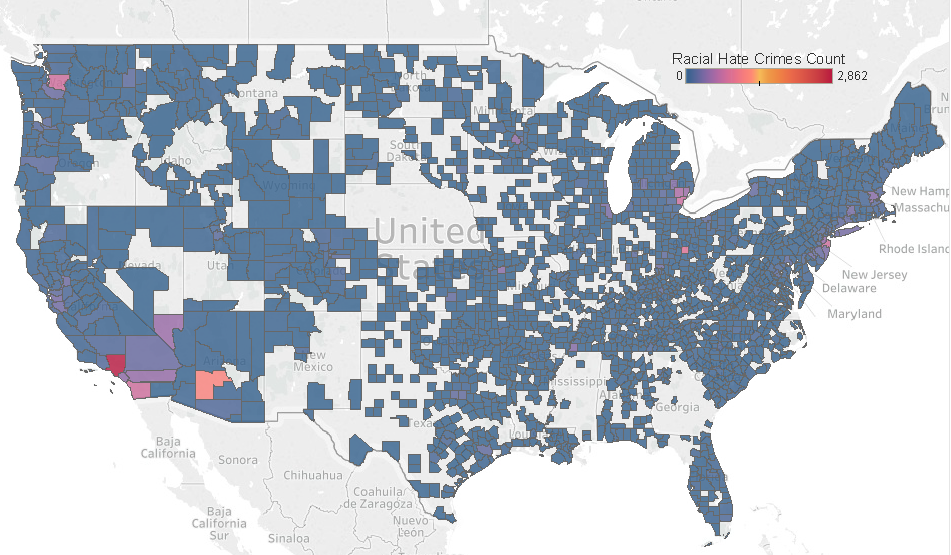
\includegraphics{/mnt/DARCE/_Research/_Cassandra Duchan/research/hate_crimes/analysis/visuals/all_hc_2005_2016.png}
\caption{All racially-motivated hate crimes by county 2005-2016}
\end{figure}

\tiny Source: United States Federal Bureau of Investigation Uniform
Crime Reporting Program Data: Hate Crime Data (Record-Type Files),
2005-2016.

\end{frame}

\begin{frame}{Geographic Distribution}

\begin{figure}
\centering
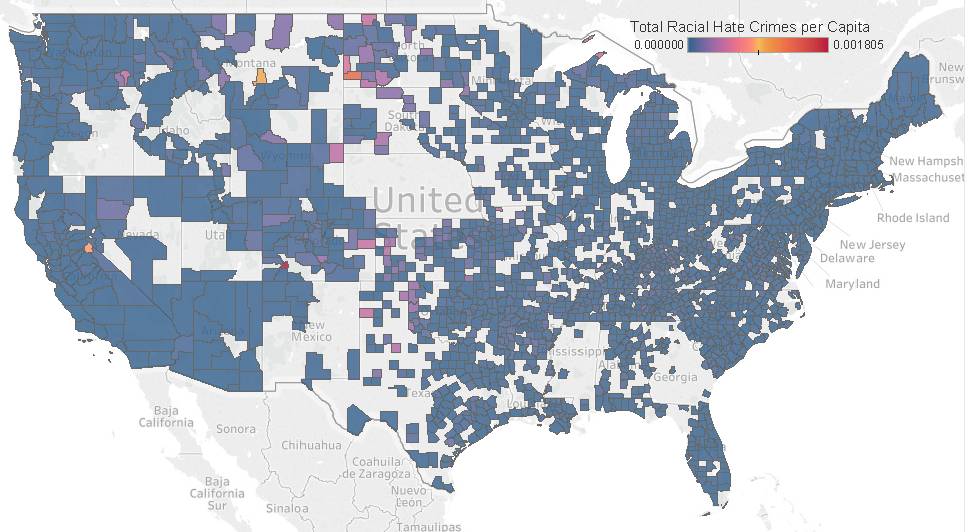
\includegraphics{/mnt/DARCE/_Research/_Cassandra Duchan/research/hate_crimes/analysis/visuals/all_hc_percap_2005_2016.png}
\caption{Racially-motivated hate crimes per capita by county 2005-2016}
\end{figure}

\tiny Source: United States Federal Bureau of Investigation Uniform
Crime Reporting Program Data: Hate Crime Data (Record-Type Files),
2005-2016.

\begin{itemize}
\tightlist
\item
  Hate crimes per capita shows a different story, with hate crimes more
  relatively prevalent in smaller counties in the middle of the US
\end{itemize}

\end{frame}

\begin{frame}{Reporting Issues}

\begin{itemize}
\tightlist
\item
  The UCR is not an exhaustive source for all hate crimes, but these
  crimes are an interesting tool for measurement because they are more
  likely to gain attention because they are reported to the police
\end{itemize}

\end{frame}

\begin{frame}{Racial or Ethnic Identity \& Ancestry}

\begin{itemize}
\tightlist
\item
  Race e.g., ``Black, African-American or Negro'', and White
\item
  Hispanic origin e.g., Different subcategories of Hispanic, Latino, or
  Spanish Origin such as Puerto Rican or Not of Hispanic, Latino, or
  Spanish Origin
\item
  Ancestry e.g., Italian, Cambodian, and Haitian

  \begin{itemize}
      \item Respondents are allowed to write in one or more ancestral responses
  \end{itemize}
\item
  In this study, each race and ethnicity is considered separately, so
  this discrepancy between race and ethnicity does not arise
\end{itemize}

\end{frame}

\begin{frame}{Methods: Presence of Any Targeted Crime}

 \[GroupIdentity_{ijt} = \\ 
    \alpha + \beta_{0} \big(AntiGroupCrime_{jt} \big) + \\
    \beta_{1}  \big( AntiGroupCrime_{jt} * GroupAncestryOnly_{ijt} \big) + \\
    \beta_{2}  \big( AntiGroupCrime_{jt} * GroupAndOtherAncestry_{ijt} \big) + \\
    X_{ijt} + \gamma_{t}  + \delta_{j} + \epsilon_{t}\]

\begin{itemize}
    \item GroupIdentity: dummy variable measuring whether individual identifies as the group targeted by a hate crime, within county j at time t 
    \item AntiGroupHateCrime: dummy indicating the presence of any group-targeted hate crime, in a given county during a given year
    \item GroupAncestry: reported ancestry comprised of either fully or half of the group targeted by a hate crime, an individual at time t
\end{itemize}

\end{frame}

\begin{frame}{Robustness Checks}

\begin{itemize}
  \item Targeted group-targeted crime per 1000 people, within county j at time t
  \item Number of group-targeted hate crimes, within county j at time t - mean of these hate crimes over the analyzed time period
\end{itemize}

\end{frame}

\end{document}
